%!TEX root = ../main.tex

\section{开胃菜}
\begin{frame}{\secname}
\vfill\hspace{20pt}
\begin{minipage}[m]{0.35\textwidth}
  \linespread{1}\large
  \tableofcontents[sectionstyle = hide/hide, subsectionstyle = show/show/hide]
\end{minipage}%
\hfill%
\begin{minipage}[m]{0.5\textwidth}
  
\includegraphics[height = 7cm]{./icons/appetizer.pdf}
\end{minipage}%
\vfill
\end{frame}

\subsection{简单的分类问题}
\begin{frame}{\insertsection}{\insertsubsection}
\begin{minipage}[m]{0.48\textwidth}
在二维空间中, 有 $500$ 个点, 这 $500$ 个点被分成两类, 一类被标记为绿色, 一类被标记为蓝色, 如右图所示.

现在的问题是, 计算机如何根据已有的数据, 找到一个分类的方法, 可以在给定 $(x_1, x_2)$ 时, 会判断点 $(x_1, x_2)$ 的颜色.

计算机解决二分类的方法有很多, 在这里, 介绍一种基于神经网络的方法, 来解决这个问题, 来帮助大家理解机器学习的过程.
\end{minipage}%
\hfill%
\begin{minipage}[m]{0.48\textwidth}
\begin{tikzpicture}
  \begin{axis}[%
    xlabel = $x_1$,
    ylabel = $x_2$,
    height = 7.8cm,
    width = 7cm,
    title = $500$ 个点的分布图
  ]
    \addplot[only marks, discard if not={type}{1}, blue] table[col sep=comma, x = x1, y = x2]{./data/classification/training_data.dat};
    \addplot[only marks, discard if not={type}{0}, green] table[col sep=comma, x = x1, y = x2]{./data/classification/training_data.dat};
  \end{axis}
\end{tikzpicture}
\end{minipage}
\end{frame}

\subsection{建立神经网络}
\begin{frame}{\insertsection}{\insertsubsection}
我们不妨设绿色为 $1$, 蓝色为 $0$, 那么, 问题就变成了找到一个坐标 $(x_1, x_2)$ 到颜色 $y$ 的一个映射关系 $y = h(x_1, x_2)$.\vspace{10pt}

\begin{minipage}[m]{0.55\textwidth}
为此, 我们建立一个简单的神经网络, 如图所示.
\begin{center}
\scalebox{0.8}{%
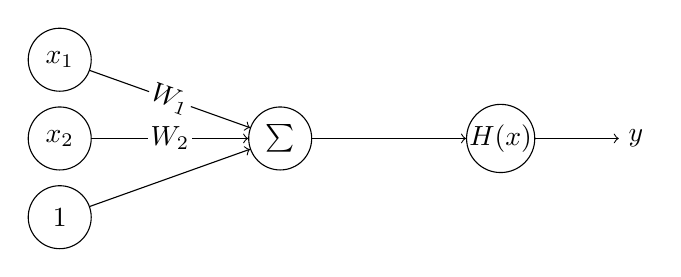
\begin{tikzpicture}[%
  node/.style = {circle, draw, inner sep = 0pt, minimum size = 0.8cm},
  x = 1.4cm]
  \node[node] (x1) at (0, 2) {$x_1$};
  \node[node] (x2) at (0, 1) {$x_2$};
  \node[node] (b)  at (0, 0) {$1$};
  \node[node] (sum) at (2, 1) {$\sum$};
  \node[node] (step) at (4, 1) {$H(x)$};

  \draw[->] (x1) -- (sum) node[midway, fill = white, inner sep = 1pt, sloped] {$W_1$};
  \draw[->] (x2) -- (sum) node[midway, fill = white, inner sep = 1pt, sloped] {$W_2$};
  \draw[->] (b) -- (sum);
  \draw[->] (sum) -- (step);
  \draw[->] (step) -- ++(0:1.5cm) node[anchor = west] {$y$};
\end{tikzpicture}}
\end{center}
因此, 我们可以得到神经网络的表达式:\vspace{-10pt}
\begin{align*}
  y &= H(W_1x_1 + W_2x_2 + 1)\text{,}\\
    &= H\big((W_1, W_2)\cdot(x_1, x_2)^\top + 1\big) = H(\bm{W}\bm{x} + 1)\text{.}
\end{align*}
\end{minipage}%
\hfill%
\begin{minipage}[m]{0.43\textwidth}
\begin{tikzpicture}
  \begin{axis}[width = \textwidth,
               height = 5.7cm,
               xlabel = $x$,
               ylabel = $H(x)$,
               title = 单位阶跃函数图像]
    \addplot[mark = none, samples = 100, blue] {x > 0};
  \end{axis}
\end{tikzpicture}
\end{minipage}
\end{frame}

\subsection{确定目标函数}
\begin{frame}{\insertsection}{\insertsubsection}
所谓目标函数, 就是当目标函数取得最值的时候, 神经网络最符合我们的预期. 换句话就是, 目标函数就是衡量神经网络好坏指标.

我们这里采用所有样本都分类成功的概率作为目标函数:
\[
p(X) = \prod_{i = 1}^{500} p(X_i)\text{,}
\]

对于第 $i$ 个坐标 $\bm{x}_i = (x_{i, 1}, x_{i, 2})$,其正确值是 $y_i$,那么当曲线 $h(x_1, x_2)$ 给定的情况下,其作出正确分类的概率为%
%
\begin{align*}
  p(X_i) &= \left\{
  \begin{array}{ll}
    1, & \text{$H(\bm{W}\bm{x}_i + 1) = 1, y_i = 1$ 或者 $H(\bm{W}\bm{x}_i + 1) = 0, y_i = 0$,}\\
    0, & \text{$H(\bm{W}\bm{x}_i + 1) = 0, y_i = 1$ 或者 $H(\bm{W}\bm{x}_i + 1) = 1, y_i = 0$.}
  \end{array}
  \right.
\end{align*}
\end{frame}

\begin{frame}{\insertsection}{\insertsubsection}
接下来, 需要对这个式子进行化简.
\[
  p(X_i) = \left\{
  \begin{array}{ll}
    1, & \text{$H(\bm{W}\bm{x}_i + 1) = 1, y_i = 1$ 或者 $H(\bm{W}\bm{x}_i + 1) = 0, y_i = 0$,}\\
    0, & \text{$H(\bm{W}\bm{x}_i + 1) = 0, y_i = 1$ 或者 $H(\bm{W}\bm{x}_i + 1) = 1, y_i = 0$.}
  \end{array}
  \right.
\]

我们可以注意到, 当 $y_i = 1$ 时, $p(X_i)$ 的值与 $H(\bm{W}\bm{x}_i + 1)$ 一致; 当 $y_i = 0$ 时, $p(X_i)$ 的值与 $H(\bm{W}\bm{x}_i + 1)$ 和为 $1$, 于是有:
\[
  p(X_i) = \left\{
  \begin{array}{ll}
    H(\bm{W}\bm{x}_i + 1), & y_i = 1\text{,}\\
    1 - H(\bm{W}\bm{x}_i + 1), & y_i = 0\text{.}
  \end{array}
  \right.
\]

注意到 $\forall x \in \mathbb{R}$ 都有 $x^0 = 1$, 还可以将上式继续化简为:
\[
  p(X_i) = H(\bm{W}\bm{x}_i + 1)^{y_i}\cdot\big(1 - H(\bm{W}\bm{x}_i + 1)\big)^{1 - y_i}\text{.}
\]
\end{frame}

\begin{frame}{\insertsection}{\insertsubsection}
因此, 我们的目标函数就确定下来了:
\[
  p(X) = \prod_{i = 1}^{500} H(\bm{W}\bm{x}_i + 1)^{y_i}\cdot\big(1 - H(\bm{W}\bm{x}_i + 1)\big)^{1 - y_i}\text{.}
\]

为了方便计算, 对上式左右两边都取以 $\e$ 为底的对数:
\[
  \ln p(X) = \sum_{i = 1}^{500} y_i\ln H(\bm{W}\bm{x}_i + 1) + (1 - y_i)\ln\big(1 - H(\bm{W}\bm{x}_i + 1)\big)\text{.}
\]

但是, 上述目标函数还存在问题:%
%
\begin{itemize}
\item 导致函数 $\ln p(X)$ 不可微, 不能采用梯度下降法来计算函数的最值(其实是极值);
\item 只要有一个预测错误, 函数 $\ln p(X) = -\infty$, 目标函数并不能衡量模型的精度.
\end{itemize}
\end{frame}

\begin{frame}{\insertsection}{\insertsubsection}
解决方法就是用 Sigmoid 函数 $g(\,\cdot\,)$ 代替上式中的单位阶跃函数 $H(\,\cdot\,)$, 原因有:
\begin{itemize}
\item Sigmoid 函数与单位阶跃函数形状非常相似, 并且值域为 $(0, 1)$, 不会导致目标函数出现 $-\infty$ 的情况, 其函数图像如右图所示.
\end{itemize}\vspace{-10pt}
\begin{minipage}[t]{0.48\textwidth}
\begin{itemize}
\item Sigmoid 处处可微, Sigmoid 的表达式为:%
\[
  g(x) = \frac{1}{1 + \exp(-x)}\text{.}
\]
\item Sigmoid 函数有非常好的导函数性质, 有:%
\[
  \frac{\dif g(x)}{\dif x} = g(x)\cdot\big(1 - g(x)\big)\text{.}
\]
\end{itemize}
\end{minipage}%
\hfill%
\begin{minipage}[t]{0.48\textwidth}
\begin{figure}
  \centering\vspace{-20pt}
  \begin{tikzpicture}
    \begin{axis}[height = 4.5cm,
                 width = \textwidth,
                 xlabel = $x$,
                 title = Sigmoid 函数与单位阶跃函数图像,
                 legend pos = north west,]
      \addplot[mark = none, blue, domain = -30:30, samples = 100] {(x > 0)};
      \addplot[mark = none, green, domain = -30:30, samples = 100] {(x <= 0) * exp(x)/(1 + exp(x)) + (x > 0) / (1 + exp(-x))};
      \legend{单位阶跃函数, Sigmoid 函数};
    \end{axis}
  \end{tikzpicture}
\end{figure}
\end{minipage}
\begin{flalign*}
& \text{目标函数:} &&  \ell(\bm{W}) = -\sum_{i = 1}^{500} y_i\ln g(\bm{W}\bm{x}_i + 1) + (1 - y_i)\ln\big(1 - g(\bm{W}\bm{x}_i + 1)\big)\text{.} &&
\end{flalign*}
\end{frame}

\subsection{参数训练}
\begin{frame}{\insertsection}{\insertsubsection}
参数训练的本质是找到一个参数 $\bm{W}$ 使目标函数 $\ell(\bm{W})$ 取得最小值, 常用的是梯度下降法.

\begin{quote}
把 $\bm{W} = (W_1, W_2)$ 看成是平面坐标, $\ell(\bm{W})$ 看作是坐标 $(W_1, W_2)$ 的海拔高度, 梯度下降法的策略就是每次向最陡的方向走一步, 一直走到海拔不变为止, 此时就是海拔``最低点'', 即 $\ell(\bm{W})$ 的极小值点.
\end{quote}\vspace{-15pt}

\tikzstyle{every picture}+=[remember picture]
\tikzstyle{na} = [baseline=-.5ex]
\begin{flalign*}
& \text{梯度下降的迭代公式为: } &&
\tikz[baseline]{\node[draw = blue, anchor = base, rounded corners] (w1) {$\bm{W}_n$};} \gets
\tikz[baseline]{\node[draw = red, anchor = base, rounded corners] (w2) {$\bm{W}_{n-1}$};} -
\tikz[baseline]{\node[draw = black, anchor = base, rounded corners] (r) {$\bm{r}$};}\cdot
\tikz[baseline]{\node[draw = green, anchor = base, rounded corners] (p) {$\dfrac{\partial \ell(\bm{W})}{\partial \bm{W}}\Big|_{\bm{W} = \bm{W}_{n-1}}$};}
\text{,}
&& \text{其中:}
\end{flalign*}

\begin{itemize}
\item 下一步的位置;\tikz[]{\node[anchor = base] (w1') {\ };}
\item 当前站的位置;\tikz[]{\node[anchor = base] (w2') {\ };}
\item 步长, 也被称为学习率;\tikz[]{\node[anchor = base] (r') {\ };}
\item 最陡的方向, 也就是梯度.\tikz[]{\node[anchor = base] (p') {\ };}
\end{itemize}

\begin{tikzpicture}[overlay]
\draw[->, rounded corners, blue] (w1') -| ([yshift = -2pt]w1.south);
\draw[->, rounded corners, red] (w2') -| ([yshift = -2pt]w2.south);
\draw[->, rounded corners, black] (r') -| ([yshift = -2pt]r.south);
\draw[->, rounded corners, green] (p') -| ([yshift = -2pt]p.south);
\end{tikzpicture}
\end{frame}

\begin{frame}{\insertsection}{\insertsubsection}
我们计算一下 $\frac{\partial \ell(\bm{W})}{\partial \bm{W}}$, 设 $z = \bm{W}\bm{x} + 1 = W_1x_{i,1} + W_2x_{i,2} + 1$, 于是:
\begin{align*}
\dfrac{\partial \ell(\bm{W})}{\partial z} &= -\dfrac{\partial \displaystyle\sum_{i = 1}^{500} \Big(y_i\ln g(z) + (1 - y_i)\ln\big(1 - g(z)\big)\Big)}{\partial z}\text{,}\\
  &= -\sum_{i = 1}^{500} y_i \dfrac{\partial \ln g(z)}{\partial z} + (1 - y_i)\dfrac{\partial\ln \big(1 - g(z)\big)}{\partial z} = -\sum_{i = 1}^{500} y_i \dfrac{g'(z)}{g(z)} + (1 - y_i)\dfrac{-g'(z)}{1 - g(z)}\text{,}\\
  &= -\sum_{i = 1}^{500} y_i \dfrac{g(z)(1 - g(z))}{g(z)} + (1 - y_i)\dfrac{-g(z)(1 - g(z))}{1 - g(z)} = -\sum_{i = 1}^{500} y_i - g(z)\text{.}\\
  \dfrac{\partial \ell(\bm{W})}{\partial W_1} &= -\dfrac{\partial \ell(\bm{W})}{\partial z} \cdot \dfrac{\partial z}{\partial W_1} = -\sum_{i = 1}^{500} \big(y_i - g(W_1x_{i,1} + W_2x_{i,2} + 1)\big)\cdot x_{i,1}\text{,}\\
  \dfrac{\partial \ell(\bm{W})}{\partial W_2} &= -\dfrac{\partial \ell(\bm{W})}{\partial z} \cdot \dfrac{\partial z}{\partial W_2} = -\sum_{i = 1}^{500} \big(y_i - g(W_1x_{i,1} + W_2x_{i,2} + 1)\big)\cdot x_{i,2}\text{.}
\end{align*}
\end{frame}

\subsection{代码实现}
\begin{frame}[fragile]{\insertsection}{\insertsubsection}
\begin{columns}
\column{\dimexpr\paperwidth-10pt}\vspace{-20pt}
\begin{pythoncode}[fontsize = \fontsize{8}{8}\selectfont]
from math import exp, log

def sigmoid(x, n = 1): # 定义 Sigmoid 函数 $g = 1/(1 + \exp(x))$
  return 1 / (1 + exp(-n * x)) if x >= 0 else exp(n * x) / (1 + exp(n * x))

def z(x1, x2, w1, w2): # 定义中间变量 $z = W_1x_1 + W_2x_2 + 1$
  return w1 * x1 + w2 * x2 + 1

def l(x1, x2, y, w1, w2): # 定义目标函数 $\ell(\bm{W}) =  -\sum_{i = 1}^{500} y_i\ln g(\bm{W}\bm{x}_i + 1) + (1 - y_i)\ln\big(1 - g(\bm{W}\bm{x}_i + 1)\big)$
  return -sum([y * log(sigmoid(z(x1, x2, w1, w2))) + (1 - y) * log(1 - sigmoid(z(x1, x2, w1, w2))) for x1, x2, y in zip(x1, x2, y)])

def get_delta_w1(x1, x2, y, w1, w2): # 定义 $\frac{\partial \ell(\bm{W})}{\partial W_1} = -\sum_{i = 1}^{500} \big(y_i - g(W_1x_{i,1} + W_2x_{i,2} + 1)\big)\cdot x_{i,1}$
  return -sum([(y - sigmoid(z(x1, x2, w1, w2))) * x1 for x1, x2, y in zip(x1, x2, y)])

def get_delta_w2(x1, x2, y, w1, w2): # 定义 $\frac{\partial \ell(\bm{W})}{\partial W_1} = -\sum_{i = 1}^{500} \big(y_i - g(W_1x_{i,1} + W_2x_{i,2} + 1)\big)\cdot x_{i,2}$
  return -sum([(y - sigmoid(z(x1, x2, w1, w2))) * x2 for x1, x2, y in zip(x1, x2, y)])
\end{pythoncode}
\end{columns}
\end{frame}

\begin{frame}[fragile]{\insertsection}{\insertsubsection}
\begin{columns}
\column{\dimexpr\paperwidth-10pt}\vspace{-20pt}
\begin{pythoncode}[fontsize = \fontsize{8}{8}\selectfont]
with open('training.dat', 'r') as data_file: # 读取训练数据 $x_1$, $x_2$ 和 $y$
  next(data_file)
  data = zip(*[[float(x.strip()) for x in line.split(',')] for line in data_file if not line.strip() == ''])
x1, x2, y = (column for column in data)

w1, w2 = 0, 0 # 初始化变量 $W_1$ 和 $W_2$
r = 0.03 # 设置学习率
precision = 1e-4 # 设置训练的目标精度

while True: # 不断的进行循环迭代, 直至 $W_1$ 和 $W_2$ 的值都不变为止
  delta_w1, delta_w2 = get_delta_w1(x1, x2, y, w1, w2), get_delta_w2(x1, x2, y, w1, w2)
  w1, w2 = w1 - r * delta_w1, w2 - r * delta_w2
  if delta_w1**2 + delta_w2**2 < precision**2:
    break

print('w1 = {w1}, w2 = {w2}'.format(w1 = w1, w2 = w2)) # 打印结果
\end{pythoncode}
\end{columns}
\end{frame}

\begin{frame}{\insertsection}{\insertsubsection}
\begin{minipage}[m]{0.32\textwidth}
在训练的过程中, 我们将每一次迭代的结果记录下来, 并绘制成曲线图, 如右图所示.

\begin{itemize}
\item 每一步的方向都是垂直于等高线, 即梯度的方向, 这就是梯度下降法的由来;
\item 步长越来越小, 这是因为坡度越来越缓;
\item 最终参数 $W_1$ 和 $W_2$ 收敛于 $(1.84, -5.46)$.
\end{itemize}
\end{minipage}%
\hfill%
\begin{minipage}[m]{0.65\textwidth}
\begin{tikzpicture}
  \begin{axis}[%
    axis equal = true,
    width = \textwidth,
    xlabel = $W_1$,
    ylabel = $W_2$,
    title = {参数 $W_1$ 和 $W_2$ 的变化轨迹}]
    \addplot[contour prepared] table[col sep=comma]{./data/classification/contour_n_equal_1.dat};
    \addplot[mark = o, mark size = 1pt] table[col sep=comma, x = w1, y = w2]{./data/classification/parameters_n_equal_1.dat};
  \end{axis}
\end{tikzpicture}
\end{minipage}
\end{frame}

\subsection{结果分析}

\begin{frame}{\insertsection}{\insertsubsection}
\begin{minipage}[m]{0.48\textwidth}
由于 参数 $W_1$ 和 $W_2$ 收敛于 $(1.84, -5.46)$, 我们可以得到一条直线:
\[
  1.84x_1 - 5.46x_2 + 1 = 0\text{.}
\]%
%
如右图所示, 可见, 结果很不理想. 通过分析数据, 我们可以看出, 点 $(1.84, -5.46)$ 处的目标函数值为 $\ell(1.84, -5.46) = 105.11$, 也是非常不理想的.

这是由于用 Sigmoid 函数代替单位阶跃函数时, 给目标函数带来的误差导致的.
\end{minipage}%
\hfill%
\begin{minipage}[m]{0.48\textwidth}
\begin{tikzpicture}
  \begin{axis}[%
    xlabel = $x_1$,
    ylabel = $x_2$,
    height = 7.8cm,
    width = 7cm,
    title = 分类效果
  ]
    \addplot[only marks, discard if not={type}{1}, blue] table[col sep=comma, x = x1, y = x2]{./data/classification/training_data.dat};
    \addplot[only marks, discard if not={type}{0}, green] table[col sep=comma, x = x1, y = x2]{./data/classification/training_data.dat};
    \addplot[mark = none, domain = -1:1, white, line width = 1pt, double = red, double distance = 2pt, on layer = foreground] {1.84/5.46*x + 1.0/5.46} node[midway, sloped, text = black] {\shadowtext{$1.84x_1 - 5.46x_2 + 1 = 0$}};
  \end{axis}
\end{tikzpicture}
\end{minipage}
\end{frame}

\subsection{改进激活函数}
\begin{frame}{\insertsection}{\insertsubsection}
\begin{minipage}[t]{0.41\textwidth}
我们对 Sigmoid 函数表达式做稍加改进, 如下所示.
\[
  g(x, n) = \frac{1}{1 + \exp(n\cdot x)}\text{.}
\]

分别绘制单位阶跃函数, $g(x, 1)$ 和 $g(x, 5)$, 可以看出, 随着 $n$ 的增大, 函数 $g(x, n)$ 越来越接近于单位阶跃函数 $H(x)$.
\end{minipage}%
\hfill%
\begin{minipage}[t]{0.55\textwidth}
\begin{figure}
  \centering\vspace{-20pt}
  \begin{tikzpicture}
    \begin{axis}[height = 6cm,
                 width = \textwidth,
                 xlabel = $x$,
                 title = Sigmoid 函数与单位阶跃函数图像,
                 legend pos = north west,]
      \addplot[mark = none, blue, domain = -10:10, samples = 100] {(x > 0)};
      \addplot[mark = none, green, domain = -10:10, samples = 100] {(x <= 0) * exp(x)/(1 + exp(x)) + (x > 0) / (1 + exp(-x))};
      \addplot[mark = none, red, domain = -10:10, samples = 100] {(x <= 0) * exp(5*x)/(1 + exp(5*x)) + (x > 0) / (1 + exp(-5*x))};

      \legend{单位阶跃函数, $1/\big(1 + \exp(x)\big)$, $1/\big(1 + \exp(5x)\big)$};
    \end{axis}
  \end{tikzpicture}
\end{figure}
\end{minipage}

\begin{flalign*}
& \text{并且可以证明:} &&
 \forall x \in \mathbb{R},\,\,\,\, \lim_{n\rightarrow +\infty} g(x, n) = \lim_{n\rightarrow +\infty}\frac{1}{1 + \exp(n\cdot x)} =  H(x)\text{.} &&
\end{flalign*}
\end{frame}

\begin{frame}{\insertsection}{\insertsubsection}
最终参数 $W_1$ 和 $W_2$ 收敛于 $(0.99, -2.93)$. 分类效果和参数 $W_1$ 和 $W_2$ 的轨迹如下所示.\vspace{10pt}

\begin{tikzpicture}
  \begin{groupplot}[group style={group size = 2 by 1, horizontal sep = 1.5cm}]
  \nextgroupplot[%
    axis equal = true,
    xlabel = $x_1$,
    ylabel = $x_2$,
    width = 0.53\textwidth,
    enlarge x limits = 0.1,
    title = 分类效果
  ]
    \addplot[only marks, discard if not={type}{1}, blue] table[col sep=comma, x = x1, y = x2]{./data/classification/training_data.dat};
    \addplot[only marks, discard if not={type}{0}, green] table[col sep=comma, x = x1, y = x2]{./data/classification/training_data.dat};
    \addplot[mark = none, domain = -1:1, white, line width = 1pt, double = red, double distance = 2pt, on layer = foreground] {0.99/2.93*x + 1.0/2.93} node[midway, sloped, text = black] {\shadowtext{$0.99x_1 - 2.93x_2 + 1 = 0$}};
  \nextgroupplot[%
    axis equal = true,
    width = 0.53\textwidth,
    xlabel = $W_1$,
    ylabel = $W_2$,
    title = {参数 $W_1$ 和 $W_2$ 的变化轨迹}]
    \addplot[contour prepared] table[col sep=comma]{./data/classification/contour_n_equal_10.dat};
    \addplot[mark = o, mark size = 1pt] table[col sep=comma, x = w1, y = w2]{./data/classification/parameters_n_equal_10.dat};
  \end{groupplot}
\end{tikzpicture}%
\end{frame}

\subsection{学习率}
\begin{frame}{\insertsection}{\insertsubsection}
\begin{minipage}[m]{0.31\textwidth}
我们把学习率 $r$ 提高, 重新进行学习, 参数 $W_1$ 和 $W_2$ 的变化轨迹如右图所示.

可以看到, 整个目标函数的最优点仍然是 $(0.99, -2.93)$, 但是, 参数 $W_1$ 和 $W_2$ 无法收敛于最优点.

相对的, 过小的学习率会导致特学习过程非常缓慢. 故选择合适大小的学习率是非常重要的.
\end{minipage}%
\hfill%
\begin{minipage}[m]{0.65\textwidth}
\begin{tikzpicture}
  \begin{axis}[%
    axis equal = true,
    width = \textwidth,
    xlabel = $W_1$,
    ylabel = $W_2$,
    title = {参数 $W_1$ 和 $W_2$ 的变化轨迹}]
    \addplot[contour prepared] table[col sep=comma]{./data/classification/contour_n_equal_10_big_learning_rate.dat};
    \addplot[mark = o, mark size = 1pt] table[col sep=comma, x = w1, y = w2]{./data/classification/parameters_n_equal_10_big_learning_rate.dat};
  \end{axis}
\end{tikzpicture}
\end{minipage}
\end{frame}

\subsection{总结}
\begin{frame}{\insertsection}{\insertsubsection}
让我们总结一下这一小节关键点:%
%
\begin{itemize}
\item 机器学习的本质是重现人认识世界的过程, 具体实现靠的是空间搜索和函数的泛化;
\item 机器学习的一般过程:
\begin{itemize}
\item 数据分析以及预处理;
\item 选择合适的模型;
\item 设定目标函数以及训练参数;
\item 验证以及调整模型.
\end{itemize}
\end{itemize}

但是, 机器学习的过程复杂, 需要计算非常复杂的目标函数, 梯度的表达式, 编码过程中非常容易出错, 训练结果难以移植到生产系统中……
\end{frame}

% \begin{frame}[fragile]{\insertsection}{\insertsubsection}
% \begin{columns}
% \column{\dimexpr\paperwidth-10pt}\vspace{-20pt}
% \begin{tcolorbox}[%
%     colback = barcolor!5!white,
%     colframe = headercolor,
%     left = 5mm,
%     top = 0pt,
%     bottom = 5pt,
%     enhanced,
% ]
% \begin{multicols}{1}
%     \begin{minted}[%
%         fontsize = \fontsize{8}{9}\selectfont,
%         linenos,
%         numbersep = 3mm,
%         autogobble,
%         breaklines,
%         breakafter = d
%     ]{python}
% from math import exp, log

% def sigmoid(x, n = 1):
%   return 1 / (1 + exp(-n * x)) if x >= 0 else exp(n * x) / (1 + exp(n * x))

% def l(x1, x2, y, w1, w2):
%   return -sum([y * log(sigmoid(z(x1, x2, w1, w2))) + (1 - y) * log(1 - sigmoid(z(x1, x2, w1, w2))) for x1, x2, y in zip(x1, x2, y)])

% def z(x1, x2, w1, w2):
%   return w1 * x1 + w2 * x2 + 1

% def get_delta_w1(x1, x2, y, w1, w2):
%   return -sum([(y - sigmoid(z(x1, x2, w1, w2))) * x1 for x1, x2, y in zip(x1, x2, y)])

% def get_delta_w2(x1, x2, y, w1, w2):
%   return -sum([(y - sigmoid(z(x1, x2, w1, w2))) * x2 for x1, x2, y in zip(x1, x2, y)])
%     \end{minted}
%   \end{multicols}
% \end{tcolorbox}
% \end{columns}
% \end{frame}
